% $Author$
% $Date$
% $Revision$

% HISTORY:
% Chapter started by Damien C (2009-09-02)

%=================================================================
\ifx\wholebook\relax\else
% --------------------------------------------
% Lulu:
	\documentclass[a4paper,10pt,twoside]{book}
	\usepackage[
		papersize={6.13in,9.21in},
		hmargin={.75in,.75in},
		vmargin={.75in,1in},
		ignoreheadfoot
	]{geometry}
	\input{../common.tex}
	\setboolean{lulu}{true}
% --------------------------------------------
% A4:
%	\documentclass[a4paper,11pt,twoside]{book}
%	\input{../common.tex}
%	\usepackage{a4wide}
% --------------------------------------------
    \graphicspath{{figures/} {../figures/}}
	\begin{document}
\fi
%=================================================================
%\renewcommand{\nnbb}[2]{} % Disable editorial comments
\sloppy
%=================================================================
\chapter{Glamour}
\chalabel{glamour}

Browsers are a crucial instrument to understand complex systems or
models. Each problem domain is accompanied by an abundance of browsers
that are created to help analyze and interpret the underlying
elements. Thee issue with these browsers is that they are frequently
rewritten from scratch, making them expensive to create and burdensome
to maintain. While many frameworks exist to ease the development of
user interfaces in general, they provide only limited support to
simplifying the creation of browsers.

Glamour is a dedicated framework to describe the navigation flow
of browsers. Thanks to its declarative language, Glamour allows to
quickly define new browsers for their data.

In this chapter we will first detail the creation of some example
browsers to have an overview of the Glamour framework. In a second
part, we will describe Glamour in more details.

\section{Installation and first browser}

To install Glamour on your \pharo{} image execute the following code:

\begin{code}{}
ScriptLoader
  loadLatestPackage: 'GlamourLoader'
  from: 'http://www.squeaksource.com/Glamour'.
(Smalltalk classNamed: #GlamourLoader) load
\end{code}

Now that Glamour is installed, we are going to build a first browser
in order to dive into Glamour's declarative language. What about
building an Apple's Finder-like file browser? This browser is built
using the Miller Columns browsing technique, displaying hierarchical
elements in a series of columns. The principle of such a browser is
that a column always reflects the content of the element selected in
the previous column, the first column-content being chosen on opening.

\damien{insert screenshot of a finder-like browser (maybe not Apple's
  finder due to license restrictions).}

In our case of implementing a file browser, we want to display a list
of a particular directory's entries (each files and directories) in
the first column and then, depending on the user selection, appending
an other column:

\begin{itemize}
\item if the user selects a directory, the next column will display
  the entries of that particular directory;
\item if the user selects a file, the next column will display the
  content of the file.
\end{itemize}

This may look complex at first. However, Glamour provides a very
simple way of describing Miller Columns-based browsers. Glamour calls
that kind of browsers finders, referring to the Apple's Finder found
on Mac OS X. To create such a browser, we are going to use the
\clsind{GLMFinder} class and then tell Glamour that we want elements
to be in a list:

\damien{SFile class and its test can be found in SLICE10146 on task forces}

\begin{code}{}
browser := GLMFinder new.
browser list
	display: [:entry | entry files].
browser openOn: SFile anyRoot.
\end{code}

From this small piece of code you get a list of all entries (either
file or directory) found at the root of your file system, each line
representing either a file or a directory. If you click on a
directory, you can see the entries of this directory in the next
column.

\damien{insert a screenshot}

This code has some problems however. Each line displays the full print
string of the entry and this is probably not what you want. A typical
user would expect only names of each entry. This can easily be done by
customizing the list:

\begin{code}{}
browser list
  display: [:entry | entry files];
  format: [:entry | entry name].
\end{code}

This way, the message \ct{name} will be sent to each entry to get its
name. This makes the files and directory much easier to read.

\damien{insert a screenshot}

Another problem is that the code does not distinguish between files
and directories. If you click on a file, you will get an error because
the browser will send it the message \ct{files} that it does not
understand. To fix that, we just have to avoid displaying a list of
contained entries if the selected element is a file:

\begin{code}{}
browser list
  display: [:entry | entry files];
  format: [:entry | entry name];
  when: [:entry | entry isDirectory].
\end{code}

This works well but the user can't distinguish between a line
representing a file or a directory. This can be fixed by, for example,
adding a slash at the end of the file name if it is a directory:

\begin{code}{}
browser := GLMFinder new.
browser list
  display: [:entry | entry files];
  format: [:entry | entry isDirectory
                                   ifTrue: [entry name, '/']
                                   ifFalse: [entry name]];
  when: [:entry | entry isDirectory].
\end{code}

The last thing we might want to do is to display the contents of the
entry if it is a file. This gives the following final code:

\begin{code}{}
browser := GLMFinder new.
browser list
  display: [:entry | entry files];
  format: [:entry | entry isDirectory
                                   ifTrue: [entry name, '/']
                                   ifFalse: [entry name]];
  when: [:entry | entry isDirectory].
browser text
	display: [:entry | [entry contents]
                                   on: Exception
                                   do: ['Can''t display the content of this file']];
	when: [:entry | entry isFile].
browser openOn: SFile anyRoot
\end{code}

\damien{insert a screenshot}

This short introduction has just presented how to install Glamour and
how to use to create a simple file browser.

\section{Tutorial: Implementing a code browser}

\damien{copy/past from thesis tutorial}

\section{Glamour in greater details}

In this section we delve into the model of Glamour. We cover Glamour's
structure and its motivations. A coarse overview of Glamour's
structure can be seen in the UML class diagram depicted in
figure~\ref{fig:uml-overview}.

\begin{figure}[htbp]
\centerline{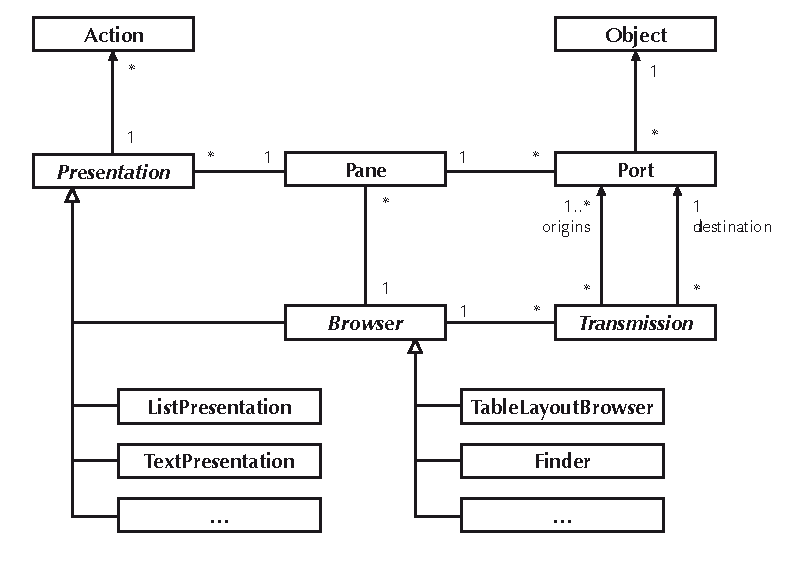
\includegraphics[width=\linewidth]{class_diagram.pdf}}
\caption{An overview of Glamour as a UML class diagram.}
\label{fig:uml-overview}
\end{figure}

\emph{Pane} defines the basic building block for browsers. A pane
consists of a number of named \emph{ports}, which can store arbitrary
data. Panes may also have one or more \emph{presentations}.

\emph{Presentations} declare a display strategy for a pane. With
presentations, panes can change their visual display on the fly. A
presentation may have units of behavior associated with them called
\emph{actions}.

\emph{Transmissions} transfer information between panes or---more accurately---their ports. When triggered, transmissions take data from one or more origin ports and deposit the data at a destination port. Two concrete subclasses of transmissions exist: \ct{SimpleTransmissions} which connect one origin to one destination and \ct{BundleTransmissions} which may have multiple origins and can set presentations on the destination pane when they are triggered.

\emph{Browsers} manage panes and transmissions. They are responsible for triggering transmissions. Browsers are themselves presentations, thus allowing them to be reused in other browsers in place of primitive presentations.

Not shown is the \emph{renderer} which implements a visitor that
transforms a composition of panes, presentations and browsers into
user interface elements that are specific to the platform and that can
be rendered on-screen or on a different medium as desired by the
user. The medium-specific transformations are specified by a concrete
subclass of \ct{GLMRenderer} such as a \ct{GLMMorphicRenderer} for
on-screen GUI elements or a \ct{SGLRenderer} to stream user interfaces
to the Seaside framework.

While class diagrams are useful for showing the relationship between
types, there is a necessity for describing \emph{instances} of
browsers and their current state. Rather than using standard UML
object diagrams, we have developed our own graphical notation. Our
abstract notation---of which an example can be seen in
figure~\ref{fig:schematic-browser}---simplifies the description and
reasoning about browsers created using the Glamour meta-model.

\begin{figure}[htbp]
\centerline{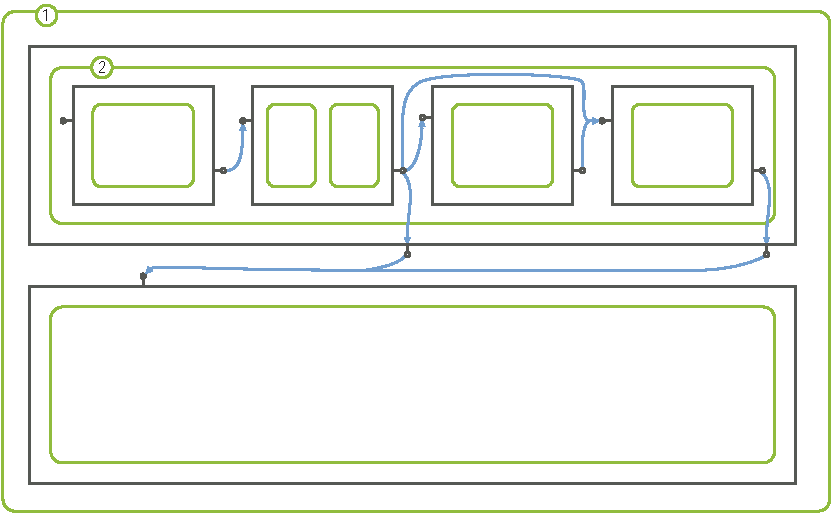
\includegraphics[width=\linewidth]{schematic_browser.pdf}}
\caption{The tutorial browser from figure~\ref{fig:mondrian-presentation} in abstract notation.}
\label{fig:schematic-browser}
\end{figure}

Figure~\ref{fig:schematic-browser} shows the abstract representation
of the class editor which we created in the tutorial section
(cf. figure~\ref{fig:mondrian-presentation}). The browser is used for
navigating through classes and their methods and consists of an outer
browser (1), that contains one pane showing the source of the
currently selected class and another pane that contains a second
browser (2) which provides panes for the packages, classes, method
categories and methods of a system. The panes (or actually their
ports) are connected using a set of directed transmissions that
describe the flow of information from one pane to another. We can see
that the basic structure of the notation resembles that of the actual
rendering of the browser.

In the following section we describe the components of a browser in
detail with the aid of our abstract browser notation. In
\ref{sec:impl/browsers-panes-transmissions} we show how browsers are
constructed and how their components are interconnected; in
\ref{sec:impl/presentations} we describe how presentations are
employed as a strategy on how to represent an underlying entity; in
\ref{sec:impl/browser-implementations} we discuss various browser
variants and the style of workflow they represent and in
\ref{sec:impl/rendering} we show how these browsers are
rendered. Finally, we discuss some specifics of the implementation in
\ref{sec:impl/smalltalk-implementation}.


%-------------------------------------------------------------------------------
\section{Browsers, Panes and Transmissions}
\label{sec:impl/browsers-panes-transmissions}

At the core, Glamour's model is a directed, possibly cyclic graph, consisting of \emph{panes} that are connected using \emph{transmissions}. This graph is encapsulated by a \emph{browser}.

The main responsibility of a pane is to store arbitrary values at named locations---its \emph{ports}. Ports have no enforced polarity or type---their interpretation depends entirely on the current \emph{presentations} of the pane which access and manipulate the pane's ports. The names usually reflect their intended use, however, such as \emph{selection} being the current selection of a list, \emph{text} holding the content being inserted into a text input, \emph{etc.} 

The \emph{transmissions} move data from one or more origin ports to one destination port. The browser acts as a broker, determining when and under which conditions transmissions should be triggered. In general, this occurs when a pane notifies its browser that one of its ports has changed its value. The browser then determines all the transmissions that originate at the port and triggers them sequentially in the order they were added to the model.

Two concrete transmission classes exist in our reference implementation. The first, \ct{SimpleTransmission}, has exactly one origin port and one destination. Simple transmissions are used whenever there is a requirement of simply copying a value from one port to another. An example of such a case is when we want to update the highlighted entity in a pane when the selection of another pane changes. When the selection of the first pane is modified, the pane notifies its containing browser which triggers the simple transmission originating at the \emph{selection} port of the first pane, which then copies the value to the \emph{highlight} port of the destination pane, effectively updating the highlighted item.

Further use cases for simple transmissions include sending port values to the outside of browsers by \emph{forwarding} them and sending values to the inside of browsers by \emph{capturing} thems (described in section~\ref{sec:impl/composition}) as well as the setting of port values by presentations contained within the pane (described in section~\ref{sec:impl/presentations}).

The second type of transmission is a \ct{BundleTransmission} which may have multiple origins but still only one destination. Bundle transmissions are the standard transmission type used between panes within a browser. They may carry a payload of a set of presentations which are inserted into the destination pane when the transmission is triggered. The use of bundle transmissions permits the modification of the representation of the pane on the fly. By making it the transmissions's responsibility to set the presentations, we maintain locality between the port values being transmitted and the presentations that will display them.

The origins of bundle transmissions are distinguished between \emph{active origins} and \emph{passive origins}. Both are specified by the developer creating the transmission. The browser will trigger the transmission whenever one of its active origins changes but not when only the port value of a passive origin changes. With passive origins, bundle transmissions are able to “pull-in” additional values that are relevant to displaying information on the destination pane.

Figure~\ref{fig:abs-browser} focuses on a subset of the abstract notation diagram that highlights these components. In the following sections we add to this sub-diagram.

\begin{figure}[htbp]
\centerline{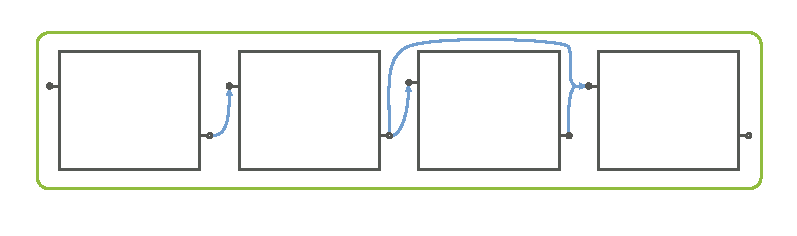
\includegraphics[width=\linewidth]{browser.pdf}}
\caption{Browsers contain panes and transmissions, which connect panes via their ports.}
\label{fig:abs-browser}
\end{figure}



%-------------------------------------------------------------------------------
\section{Presentations}
\label{sec:impl/presentations}

Presentations provide visual semantics to the state of panes. They read and interpret the values of selected ports---known as \emph{input ports}---and, in turn, may choose to populate a set of other ports with values---the \emph{output ports}.

A pane can have no presentation, a single presentation or multiple presentations at any given moment. Multiple presentations are usually displayed with the use of a tab panel. As the state is encapsulated by the pane, multiple presentations on the same pane will share that same state. In our abstract notation, presentations are displayed within their panes as depicted in figure~\ref{fig:abs-presentations}.

\begin{figure}[htbp]
\centerline{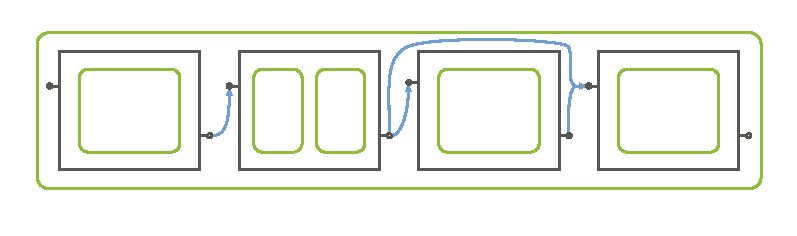
\includegraphics[width=\linewidth]{presentations.pdf}}
\caption{Presentations interpret and modify the state of their pane by reading from and writing to its ports.}
\label{fig:abs-presentations}
\end{figure}

Various concrete subclasses of presentation exist and are usually named after their recommended visual representation. For example, \ct{ListPresentation} is rendered as a list user interface widget, \ct{TextPresentation} as a text input. The concrete representation is not encoded within the presentation class due to the intentional separation of widget-toolkit specific behavior from our model. However, the renderers which create the user interface elements heed the suggested representation and render the presentation accordingly. In return, presentations provide a well-defined and extensive interface to the rendering client to avoid that renderers directly access or manipulate the pane and its ports to reflect changes of the user interface. This prevents coupling as the renderers do not have to access the state of the presentations directly but rely solely on a higher-level and well defined interface.

The presentations implement a strategy pattern \cite{Gamm95a} that uses a pane as its context object as is shown in figure~\ref{fig:uml-strategy}. It allows us to change the behavior of the pane on the fly and dynamically apply a new filter. This has the advantage that the communication structure determined by the panes and components can be statically defined for a particular browser, but the representation can be dynamically changed depending on the particular instance in the domain model that is currently being displayed.

\begin{figure}[htbp]
\centerline{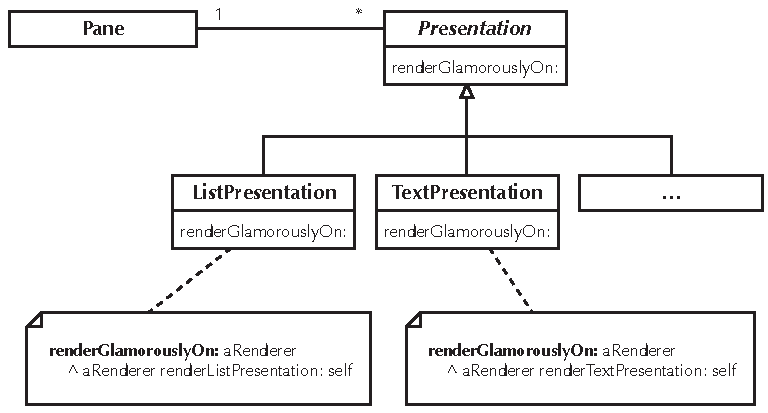
\includegraphics[width=\linewidth]{uml_strategy.pdf}}
\caption{UML displaying how presentation strategies are employed by panes.}
\label{fig:uml-strategy}
\end{figure}


%-------------------------------------------------------------------------------
\section{Actions}
\label{sec:impl/actions}

All presentations can be configured with a number of \emph{actions}. Actions encapsulate units of behavior that can be executed upon the presentation or its corresponding panes. They may also be associated with a string name or a keyboard shortcut. The concrete representation of the actions lies in the responsibility of the renderer which may choose to simply trigger them when a key-combination is pressed on the keyboard or display them as a context menu to the widget that the presentation is associated with.

A frequent application for actions is to create a menu item or a keyboard shortcut that triggers a navigation, much like clicking on an item in a list may results in a navigation. The solution is to create an action that populates a port which is then connected to a destination pane using a normal transmission. When the action is executed, the port value changes, thus causing a navigation.


%-------------------------------------------------------------------------------
\section{Composition}
\label{sec:impl/composition}

Browsers in Glamour can be composed by treating presentations and browsers equally. In fact, browser \emph{are} presentations as one can see from our class diagram in figure~\ref{fig:uml-overview}. This means that, anywhere a list presentation or other type of primitive presentation may be used, a browser can be substituted instead. This simplifies the declaration of browsers in Glamour and promotes their reuse.

One major difference to a typical composition pattern rests in the use of the strategy pattern for presentations as discussed above. Since panes contain presentations and browsers contain panes (which are themselves presentations), the composition of browsers results in an indirect nesting as exemplified in the alternating chain shown in figure~\ref{fig:uml-object-chain}.

\begin{figure}[htbp]
\centerline{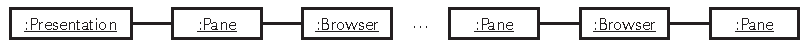
\includegraphics[width=\linewidth]{uml_object_chain.pdf}}
\caption{UML object diagram showing how components are composed.}
\label{fig:uml-object-chain}
\end{figure}


With composed browsers, it is often a requirement to access port values of panes that are within browsers from outside that browser. The motivation for such behavior in our class editor was discussed in the tutorial chapter (see figure~\ref{sec:tutorial/reusing-browsers}). To meet this requirement, the value of a port can be forwarded to another port. The usage of such forwarding to export values to the outside of a browser is shown in figure~\ref{fig:abs-port_publishing}

\begin{figure}[htbp]
\centerline{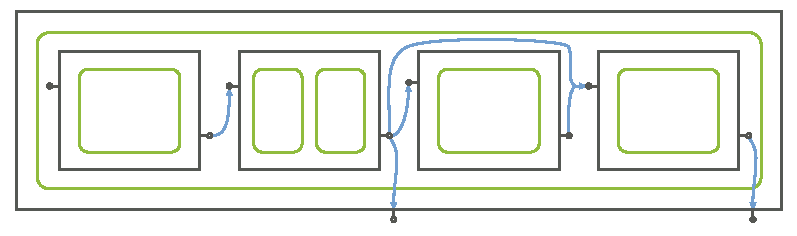
\includegraphics[width=\linewidth]{portpublishing.pdf}}
\caption{A browser forwards a port of one of its panes to its containing pane so that its value can be accessed from outside.}
\label{fig:abs-port_publishing}
\end{figure}

It is noteworthy that this forwarding of information is implemented as a standard \emph{simple transmission}, managed by the inner browser. Whenever the origin port changes, the pane will inform the browser of this, triggering the transmissions originating at the port. As the browser's outer pane---and with it the destination port of the forwarding transmissions---may vary at runtime as the browser is deployed and removed from various panes, the destination port of a forwarding transmission is a \emph{lazily evaluated} port. A lazily evaluated port is resolved to an actual port at the point where the transmission is fired.

Just as port values can be forwarded to an outside pane, browsers can also capture port value changes on the encapsulating pane and forward these to an inner port. This would essentially be the reversal of the direction of the arrows to the outside shown in figure \ref{fig:abs-port_publishing}. The purpose of this type of capturing would be to allow certain properties of a browser---such as the selection or the highlighted item of a specific pane---to be modified from the outside.



%-------------------------------------------------------------------------------
\section{Browser Implementations}
\label{sec:impl/browser-implementations}

The exact handling of panes and transmissions depends on a concrete subclass of browser. Several types of browsers exist but we can differentiate between two general categories: browsers with \emph{explicit} pane configurations and browser with \emph{implicit} pane configurations. In the first case, panes must be declared and configured by the user and usually remain static at runtime. In the second case, the browser creates and destroys panes as needed. We provide an example for each.

The \ct{TableLayoutBrowser} requires its panes to be explicitly declared and is named after the ability to customize the layout of its panes. The browser is configured with a number of rows or columns which then may be subdivided in columns or rows respectively. Each cell that is defined in this way represents a pane and is given a unique name.

An example of a browser which uses implicit pane configurations is the \emph{finder} which implements a \emph{Miller Columns} style browsing. The browser starts by displaying only one pane. When the selection changes within this pane, the browser will create a new pane to the right, connect the two panes using a transmission and fire the transmission to populate the new pane. This process is always repeated for the rightmost pane. When the selection changes for a pane that is not the last one in the list, all panes to the right will first be destroyed before creating a new pane.



%-------------------------------------------------------------------------------
\section{Rendering}
\label{sec:impl/rendering}

In our reference implementation we have created two concrete renderers: \ct{WidgetryRenderer} builds a representation of browsers using the Widgetry GUI library in VisualWorks and \ct{GlareRenderer} registers a Glare application \cite{Bunge08a} that streams the user interface to an Adobe Flex client over a network connection.

A renderer acts as a \emph{visitor} \cite{Gamm95a} that traverses the component tree of browsers, panes and presentations, creating appropriate user interface elements for the components it encounters. As these elements are created, the renderer is also responsible for connecting the appropriate library-dependent callbacks to populate panes and their ports with the appropriate values when actions are performed or the state of the user interface components changes.

In \ct{GlareRenderer} for example, selecting an item within a list widget triggers a callback that sets the value of the \emph{selection} port of the corresponding pane. Double clicking populates the \emph{execution} port and hovering over an item sets the value of the \emph{hover} port. Different widgets might set other port values and some renderer implementations may choose not to support hovering or other operatives at all. Nevertheless, renderers do not communicate with the pane directly and use only the interface given to them by the presentation. This helps renderers to work in a consistent and predictable way. A user writing a browser would not expect that in one rendition of a model the selection of an item in the list would result in the setting of \emph{selection} and in another in the setting of \emph{choice}.

Developers wishing to create user interface elements for other environments need only create a new subclass of \ct{Renderer} and implement the appropriate methods. An incomplete list of these is shown in figure~\ref{fig:renderer}. Due to their similarity, the existing renderers may serve as a guide in determining the expected behavior of new implementations.

\begin{figure}[htbp]
\centerline{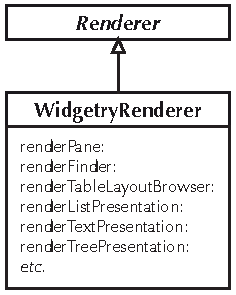
\includegraphics[width=\linewidth]{renderer.pdf}}
\caption{A subclass of renderer and some of the implemented methods.}
\label{fig:renderer}
\end{figure}


%-------------------------------------------------------------------------------
\section{Smalltalk Implementation}
\label{sec:impl/smalltalk-implementation}

While our core contribution is the meta-model, we have also developed a declarative language in our reference implementation to construct specific browser models. The declarative language of Glamour is implemented as an internal domain specific language \cite{Fowl07c} (also known as an embedded DSL \cite{Huda98a}) that uses Smalltalk as its host language.

In our language implementation, we make heavy use of Smalltalk's features such as block closures and cascades. Take for example the following code snippet:

\begin{code}{}
browser showOn: #classes; from: #pundles; using: [
	browser list
		display: [ :pundle | pundle containedClasses ];
		when: [ :pundle | pundle isPackage ].
	browser mondrian painting: [ ... ]
].
\end{code}

The block closure argument passed to \ct{using:} ensures that the contained list of presentations belong to the same transmission. We use cascades as with \ct{display:} and \ct{when:} to pass multiple options to the same object---a presentation in this example. Block closures are also used to define anonymous callbacks for these arguments, such as the filter condition in when or the display block. 

Rather than building an intermediate representation our declarative language works directly on the Glamour model. When we call \ct{browser list} for example, our script tells the browser to add a new list presentation to the latest transmission and returns that presentation so that \ct{display:} and \ct{when:} can be sent to it. To facilitate this, our scripting language is implemented as a set of \emph{class extensions} to the core model. We use extensions rather than implementing the methods in the classes directly to provide some separation between the programmatic and the scripting interfaces, and thus to improve maintainability. Figure~\ref{fig:uml-script_extensions} shows a selection of the class extensions introduced by the scripting implementation.

\begin{figure}[htbp]
\centerline{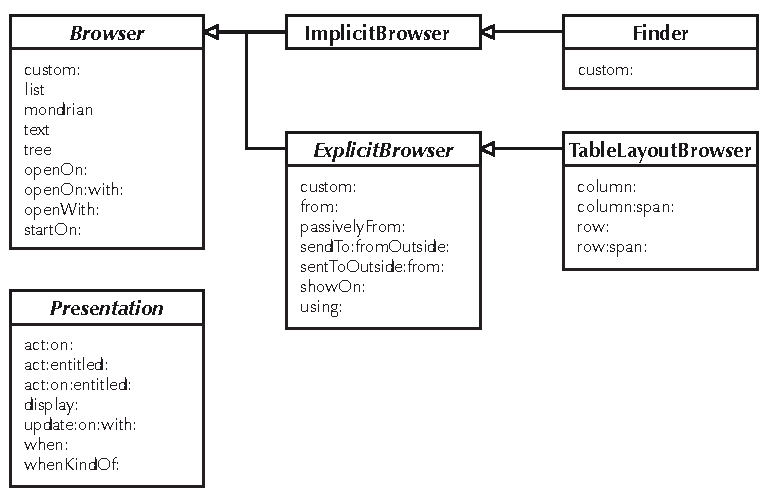
\includegraphics[width=\linewidth]{script_extensions.pdf}}
\caption{Class extensions made by the scripting language implementation.}
\label{fig:uml-script_extensions}
\end{figure}

The most interesting method shown above is the \ct{custom:} message. Sending this message adds a \emph{custom presentation} to the current context of the browser. The \ct{list}, \ct{text}, \ct{tree}, and \ct{mondrian} messages are just convenience messages that call \ct{custom:} with an appropriate presentation instance. For example, the \ct{list} message is implemented as follows:

\begin{code}{}
list
	^ self custom: ListPresentation new.
\end{code}

Most of the extensions are quite straightforward, simply calling their programatic equivalent on the model. To add an action to a presentation for example, the \ct{act:on:} message is implemented as:

\begin{code}{}
act: aBlock on: aCharacter 
	self addAction: (Action new
		action: aBlock;
		shortcut: aCharacter;
		yourself)
\end{code}

The list of messages is evolving and some are added simply for convenience to the developer. An example is the navigate-upon-action mechanism described in \ref{sec:impl/actions} where the pressing of a keyboard shortcut or the clicking of a menu item triggers a navigation within the browser. Since this is such a common requirement, our reference implementation provides the dedicated message:
\begin{quotation}\noindent
\lstinline{update: aPortSymbol on: aCharacter with: aBlock}
\end{quotation}

Whenever the shortcut key defined by \ct{aCharacter} is pressed, the message causes the port named by \ct{aPortSymbol} to be updated with the result of evaluating \ct{aBlock}, whose arguments are described in \ref{sec:tutorial/actions}. Similar messages with \ct{entitled:} are available for defining menu entries.

The following example shows how this mechanism is used to navigate to either the subclasses or the superclass of a selected class when a particular shortcut is pressed:

\begin{code}{}
browser showOn: #classes; using: [
	browser list
		update: #relatedClass on: $b with: [ :list |
			list selection subclasses ].
		update: #relatedClass on: $p with: [ :list |
			Array with: list selection superclass ]
].

browser showOn: #relatedClasses;
	from: #classes -> #relatedClass; using: [
	browser list
].
\end{code}


%-------------------------------------------------------------------------------
\section{Model Implementations}

In addition to our VisualWorks reference implementation, Glamour has attracted the interest of other researchers who work on other platforms. Tudor Gîrba, Lukas Renggli and David Röthlisberger have successfully ported Glamour to the Pharo Smalltalk dialect. The code base is taken largely from the reference implementation but other renderers have been implemented to fit the environment. As Pharo primarily uses the direct-manipulation user interface \emph{Morphic} to represent its widgets, building a corresponding visitor for Glamour was required. Additionally, a renderer for the Seaside web application framework has been written which renders Glamour models using a combination of basic HTML components and asynchronous Javascript (AJAX).

Probably the most important result of this work for us is that the researchers found it easy to write additional renderers. It provides additional justification for separating the rendering from our model and shows that the added complexity arising from this separation is reasonable.



%=============================================================
\ifx\wholebook\relax\else
   \bibliographystyle{jurabib}
   \nobibliography{scg}
   \end{document}
\fi
%=============================================================




%-----------------------------------------------------------------

%%% Local Variables:
%%% coding: utf-8
%%% mode: latex
%%% TeX-master: t
%%% TeX-PDF-mode: t
%%% ispell-local-dictionary: "english"
%%% End: